\chapter{LITERATURE STUDY}
\label{chap:literaturestudy}

% Ubah bagian-bagian berikut dengan isi dari tinjauan pustaka

This chapter will explain the supporting theories that are used as references for this study.
The theories described in this chapter will be presented in a systematic order, starting from the most basic
to deeper explanations.

\section{Pose Estimation}
\label{sec:poseestimation}

% Contoh input gambar
\begin{figure}[ht]
  \centering

  % Ubah dengan nama file gambar dan ukuran yang akan digunakan
  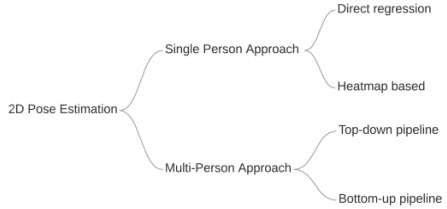
\includegraphics[scale=1]{gambar/taxonomy-pose-estimation.png}

  % Ubah dengan keterangan gambar yang diinginkan
  \caption{Taxonomy of pose estimation approaches}
  \label{fig:pose-estimation}
\end{figure}

Pose estimation is a heavily explored area with applications in gaming, animation, action recognition, activity tracking, and augmented reality.
In order to improve pose estimate outcomes, various approaches have been developed. These methods may generally be split into: Single-person and Multi-person approaches, 
as depicted in figure \ref{fig:pose-estimation}. The single-person approach is fundamentally a regression issue because it just determines the pose of a single person in an image, 
the person's position and an implicit number of keypoints are already known. However, the multi-person approach tries to solve an unconstrained problem because we do not know 
the positions and number of persons within the image \parencite{romeo}.

The single-person approach is divided into two frameworks based on the keypoint prediction method: directly regressing keypoints from the features (i.e. direct regression based framework)
or by generating heatmaps and inferencing keypoints via heatmap (i.e. heatmap based framework) \parencite{romeo}.
A direct regression-based framework can be implemented in various ways: as done by \parencite{toshev2014}, 
they presented DeepPose where their model uses a simple architecture with a convolutional layer, followed by a dense layer that will produce keypoint values in \emph{(x,y)}.
Other authors \parencite{carreira2015} suggested a technique that iteratively improves model output by feeding back mistake predictions, leading to a notable improvement in accuracy.

Then for a heatmap based framework, an alternative method can be used to generate heatmaps of all keypoints in the image
rather than directly predicting them. The final stick figure is then created using additional techniques to know the connection between keypoints or joints.
In \parencite{chen2014}, authors proposed a graphical model with pairwise
relations to make adaptive use of local image measurements. Later on, both the detection of joints and the prediction of their relationships can be accomplished using those local image measurements.
\parencite{newell2016} designed a \emph{"stacked hourglass"} network, that is closely similar to encoder-decoder architecture and is based on the sequential phases of pooling and upsampling.
They demonstrated the importance of repeated bottom-up, top-down processing with intermediate supervision for enhancing the effectiveness of human pose detection.

The multi-person approach is a more complex task because
the positions and number of persons within the image are unknown, therefore the framework has to detect keypoints and assemble an unknown number of persons. To overcome this task,
two pipelines have been proposed: top-down pipeline and bottom-up pipeline \parencite{romeo}.
Beginning with the detection of every person present in an image, the top-down pipeline creates bounding boxes. The following action uses each of the identified bounding boxes and applies a single-person method. 
For each person that is discovered, the single-person technique will generate keypoints, and then, as shown in figure \ref{fig:top-down-approach}, the pipeline may include extra steps of post-processing and improving final results.

\begin{figure}[ht]
  \centering
  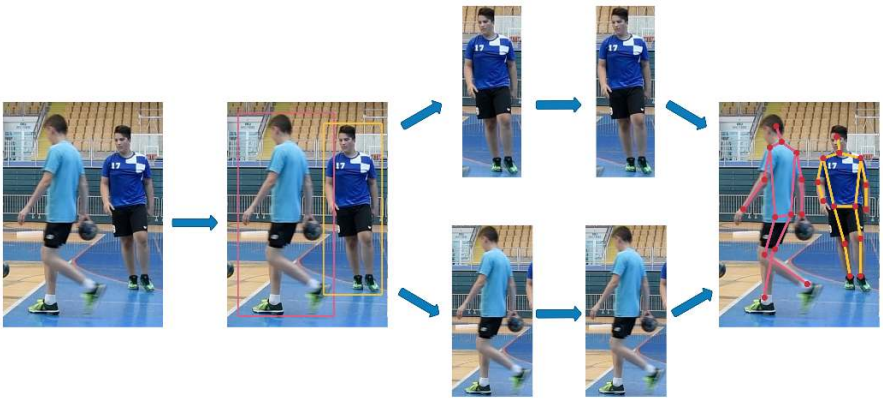
\includegraphics[scale=0.7]{gambar/top-down-approach.png}
  \caption{The top-down pipeline in multi-person approach for pose estimation}
  \label{fig:top-down-approach}
\end{figure}

Compare to a top-down pipeline, the bottom-up pipeline operates in reverse. The bottom-up pipeline begins by finding all of the keypoints, which are then connected to human instances, as seen in figure \ref{fig:bottom-up-approach}. 
The bottom-up pipeline is probably quicker than the top-down pipeline because it doesn't detect human bounding boxes and runs pose estimation for each person individually.

\begin{figure}[ht]
  \centering
  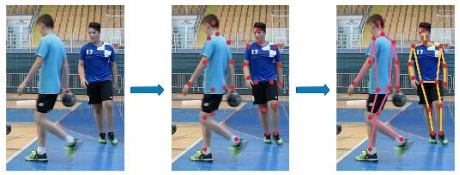
\includegraphics[scale=1]{gambar/bottom-up-approach.png}
  \caption{The bottom-up pipeline in multi-person approach for pose estimation.}
  \label{fig:bottom-up-approach}
\end{figure}

\section{Gravitasi}
\label{sec:gravitasi}

Gravitasi merupakan \lipsum[1]

\subsection{Hukum Newton}
\label{subsec:hukumnewton}

Newton \parencite{newton1687} pernah merumuskan bahwa \lipsum[1]
Kemudian menjadi persamaan seperti pada persamaan \ref{eq:hukumpertamanewton}.

% Contoh pembuatan persamaan
\begin{equation}
  \label{eq:hukumpertamanewton}
  \sum \mathbf{F} = 0\; \Leftrightarrow\; \frac{\mathrm{d} \mathbf{v} }{\mathrm{d}t} = 0.
\end{equation}

\subsection{Anti Gravitasi}
\label{subsec:antigravitasi}

Anti gravitasi merupakan \lipsum[1]
